\documentclass[norsk, doc, 11pt, a4paper]{apa7}  % defines the basic parameters of the document
% if you want a single-column, remove reprint

% allows special characters (including æøå)
\usepackage[norsk]{babel}
\usepackage[utf8]{inputenc}

\usepackage{csquotes}
\usepackage[style=apa, backend=biber]{biblatex}

%% note that you may need to download some of these packages manually, it depends on your setup.
%% I recommend downloading TeXMaker, because it includes a large library of the most common packages.

\usepackage{physics,amssymb}  % mathematical symbols (physics imports amsmath)
\usepackage{graphicx}         % include graphics such as plots
\usepackage{xcolor}           % set colors
\usepackage{hyperref}         % automagic cross-referencing (this is GODLIKE)
\usepackage{tikz}             % draw figures manually
\usetikzlibrary{tikzmark}
\usepackage{listings}         % display code
\usepackage{cprotect}
\usepackage{float}
\usepackage{caption}
\usepackage{subcaption}
\usepackage{xpatch}

%\setlength{\parindent}{0px}

%Ta med disse kommandoene
\newcommand{\nnode}[2]{\node (#1) at (#2) {#1};}    %Her defineres nnode kommandoen
\newcommand{\relnode}[2]{\draw (#2) node[fill,circle,scale=0.6]{} (#2);\node (#1) at (#2) {};}  %Her defineres relnode kommandoen

% defines the color of hyperref objects
% Blending two colors:  blue!80!black  =  80% blue and 20% black
\hypersetup{ % this is just my personal choice, feel free to change things
    colorlinks,
    linkcolor={red!50!black},
    citecolor={blue!50!black},
    urlcolor={blue!80!black}}
%
%% Defines the style of the programming listing
%% This is actually my personal template, go ahead and change stuff if you want
\lstnewenvironment{python}{
	\lstset{ %
		inputpath=,
		backgroundcolor=\color{white!95!black},
		basicstyle={\ttfamily\scriptsize},
		commentstyle=\color{orange},
		language=Python,
		%numbers=left,
		%stepnumber=1,
		morekeywords={True,False},
		tabsize=4,
		stringstyle=\color{green!55!black},
		frame=single,
		keywordstyle=\color{blue},
		showstringspaces=false,
		columns=fullflexible,
		keepspaces=true,
		upquote=true}
}{}

\lstnewenvironment{cpp}{
	\lstset{ %
		inputpath=,
		backgroundcolor=\color{white!95!black},
		basicstyle={\ttfamily\scriptsize},
		commentstyle=\color{orange},
		language=C++,
		%numbers=left,
		%stepnumber=1,
		morekeywords={True,False},
		tabsize=4,
		stringstyle=\color{green!55!black},
		frame=single,
		keywordstyle=\color{blue},
		showstringspaces=false,
		columns=fullflexible,
		keepspaces=true,
		upquote=true}
}{}

\lstnewenvironment{csharp}{
	\lstset{ %
		inputpath=,
		backgroundcolor=\color{white!95!black},
		basicstyle={\ttfamily\scriptsize},
		commentstyle=\color{orange},
		language=[Sharp]C,
		%numbers=left,
		%stepnumber=1,
		morekeywords={True,False},
		tabsize=4,
		stringstyle=\color{green!55!black},
		frame=single,
		keywordstyle=\color{blue},
		showstringspaces=false,
		columns=fullflexible,
		keepspaces=true,
		upquote=true}
}{}

\lstnewenvironment{sql}{
	\lstset{ %
		inputpath=,
		backgroundcolor=\color{white!95!black},
		basicstyle={\ttfamily\scriptsize},
		commentstyle=\color{orange},
		language=SQL,
		%numbers=left,
		%stepnumber=1,
		morekeywords={True,False},
		tabsize=4,
		stringstyle=\color{green!55!black},
		frame=single,
		keywordstyle=\color{blue},
		showstringspaces=false,
		columns=fullflexible,
		keepspaces=true,
		upquote=true}
}{}

\lstnewenvironment{mongodb}{
	\lstset{ %
		inputpath=,
		backgroundcolor=\color{white!95!black},
		basicstyle={\ttfamily\scriptsize},
		commentstyle=\color{orange},
		language=bash,
		%numbers=left,
		%stepnumber=1,
		morekeywords={True,False},
		tabsize=4,
		stringstyle=\color{green!55!black},
		frame=single,
		keywordstyle=\color{blue},
		showstringspaces=false,
		columns=fullflexible,
		keepspaces=true,
		upquote=true}
}{}

\lstnewenvironment{php}{
	\lstset{ %
		mathescape=false,
		inputpath=,
		backgroundcolor=\color{white!95!black},
		basicstyle={\ttfamily\scriptsize},
		commentstyle=\color{orange},
		language=php,
		%numbers=left,
		%stepnumber=1,
		morekeywords={True,False},
		tabsize=4,
		stringstyle=\color{green!55!black},
		frame=single,
		keywordstyle=\color{blue},
		showstringspaces=false,
		columns=fullflexible,
		keepspaces=true,
		upquote=true}
}{}


%\lstset{literate=
%  {á}{{\'a}}1 {é}{{\'e}}1 {í}{{\'i}}1 {ó}{{\'o}}1 {ú}{{\'u}}1
%  {Á}{{\'A}}1 {É}{{\'E}}1 {Í}{{\'I}}1 {Ó}{{\'O}}1 {Ú}{{\'U}}1
%  {à}{{\`a}}1 {è}{{\`e}}1 {ì}{{\`i}}1 {ò}{{\`o}}1 {ù}{{\`u}}1
%  {À}{{\`A}}1 {È}{{\'E}}1 {Ì}{{\`I}}1 {Ò}{{\`O}}1 {Ù}{{\`U}}1
%  {ä}{{\"a}}1 {ë}{{\"e}}1 {ï}{{\"i}}1 {ö}{{\"o}}1 {ü}{{\"u}}1
%  {Ä}{{\"A}}1 {Ë}{{\"E}}1 {Ï}{{\"I}}1 {Ö}{{\"O}}1 {Ü}{{\"U}}1
%  {â}{{\^a}}1 {ê}{{\^e}}1 {î}{{\^i}}1 {ô}{{\^o}}1 {û}{{\^u}}1
%  {Â}{{\^A}}1 {Ê}{{\^E}}1 {Î}{{\^I}}1 {Ô}{{\^O}}1 {Û}{{\^U}}1
%  {œ}{{\oe}}1 {Œ}{{\OE}}1 {æ}{{\ae}}1 {Æ}{{\AE}}1 {ß}{{\ss}}1
%  {ű}{{\H{u}}}1 {Ű}{{\H{U}}}1 {ő}{{\H{o}}}1 {Ő}{{\H{O}}}1
%  {ç}{{\c c}}1 {Ç}{{\c C}}1 {ø}{{\o}}1 {å}{{\r a}}1 {Å}{{\r A}}1
%  {€}{{\euro}}1 {£}{{\pounds}}1 {«}{{\guillemotleft}}1
%  {»}{{\guillemotright}}1 {ñ}{{\~n}}1 {Ñ}{{\~N}}1 {¿}{{?`}}1
%}

\newcommand{\set}[1]{\ensuremath{\left\{#1\right\}}}
\newcommand{\tuple}[1]{\ensuremath{\left\langle #1 \right\rangle}}
\newcommand{\imp}{\ensuremath{\rightarrow}}

\newcommand{\ceil}[1]{\ensuremath{\lceil #1 \rceil}}
\newcommand{\floor}[1]{\ensuremath{\lfloor #1 \rfloor}}

\usepackage{thmtools}
\DeclareMathOperator{\nullspace}{Nul}
\DeclareMathOperator{\collspace}{Col}
\DeclareMathOperator{\rref}{Rref}
%%\DeclareMathOperator{\dim}{Dim}

 % "meq": must be equal
\newcommand{\meq}{\overset{!}{=}}
\newcommand\numberthis{\addtocounter{equation}{1}\tag{\theequation}}

\newcommand{\R}{\mathbb{R}}
\newcommand{\N}{\mathbb{N}}
\newcommand{\Z}{\mathbb{Z}}
\newcommand{\Q}{\mathbb{Q}}
\newcommand{\C}{\mathbb{C}}
\newcommand*\Heq{\ensuremath{\overset{\kern2pt L'H}{=}}}
\usepackage{bm}
\newcommand{\uveci}{{\bm{\hat{\textit{\i}}}}}
\newcommand{\uvecj}{{\bm{\hat{\textit{\j}}}}}
\newcommand{\uveck}{{\bm{\hat{\textit{\k}}}}}

\DeclareRobustCommand{\uvec}[1]{{%
  \ifcsname uvec#1\endcsname
     \csname uvec#1\endcsname
   \else
    \bm{\hat{\mathbf{#1}}}%
   \fi
}}
\usepackage[binary-units=true]{siunitx}

\newcommand{\twopartdef}[4]
{
	\left\{
		\begin{array}{ll}
			#1 & \mbox{if } #2 \\
			#3 & \mbox{if } #4
		\end{array}
	\right.
}

\makeatletter
\xpatchcmd{\appendix}
  {\par}
  {\addcontentsline{toc}{section}{\@currentlabelname}\par}
  {}{}
\makeatother

\makeatletter
\newcommand*{\balancecolsandclearpage}{%
  \close@column@grid
  \cleardoublepage
  \twocolumngrid
}
\makeatother

\AtBeginEnvironment{align}{\setcounter{equation}{0}}
\newcounter{subproject}
\renewcommand{\thesubproject}{\alph{subproject}}
\newenvironment{subproj}{
\begin{description}
	\item[\refstepcounter{subproject}(\thesubproject)]
}{\end{description}}

\addbibresource{referanser.bib}

\title{Mappeoppgave Visualisering og Simulering}   % self-explanatory
\author{Kandidatnummer: 843}               % self-explanatory
\affiliation{Høgskolen i Innlandet}
\date{\today}                             % self-explanatory
\shorttitle{VSIM101 | kandidat.nr.: 843}
%\noaffiliation                            % ignore this


\abstract{Jeg har implementert prosessering av punktskydata i C++, og simulering av regn og ball på trekantflate basert på punktskydata i Unity 2022.3.7f1. Prosjektet er tilgjengelig her: \url{https://github.com/FunkMarvel/VisSimMappe.git} .}

\begin{document}
\maketitle                                % creates the title, author, date
\tableofcontents

\section{Introduksjon}
Et viktig aspekt av moderne beredskap er forståelsen av ekstremvær og dets effekt på lokal natur. Derfor er det nødvendig å kunne lage digitale representasjoner av virkelige terreng, samt simulere fysikk ved bruk av datamaskin på slike representasjoner. I denne rapporten utforsker jeg en metode for å modellere, samt simulere effekten av nedbør på terreng konstruert fra punktskydata.

Rapporten fokuserer på hvordan lage en regulært indeksert trekantflate som representerer terrenget, samt hvordan bruke B-Splines til å kartlegge vassdrag som dannes ved ekstrem nedbør, og hvordan simulere effekten et slik vassdrag har på løsmateriale.

\section{Metode}
\subsection{Punktsky og triangulering}
\subsubsection{Vertekser} \label{M:1:1}
Moderne målinger av terreng gjøres med LiDAR, og resulterer i rådata i form av en uorganisert samling punkter i \(\R^{3}\) relativt til et valgt koordinatsystem \parencite{bergerSurveySurfaceReconstruction2017}. Jeg har valgt å laste ned punktdata fra Kartverket sin database '\url{hoydedata.no}' i '.laz'-format, som jeg så konverterer til en rentekst-fil ved hjelp av programvaren 'LASzip' \parencite{isenburgLASzip2019}. Høydedataene er fra følgende målinger: \parencite{HoydedataNDHEngerdal2018, HoydedataNDHEngerdal2018a, HoydedataNDHTrysil2018}. Den resulterende tekstfilen fra LASzip inneholder da \(n\) antall punkter fordelt på formen
\begin{align*}
 x_{0} \quad &y_{0} \quad z_{0} \\
 x_{1} \quad &y_{1} \quad z_{1} \\
 ... \quad &... \quad ... \\
 x_{n-1} \quad &y_{n-1} \quad z_{n-1}
\end{align*}
hvor hver linje svarer til et punkt.
\begin{figure}[H]
	\centering
	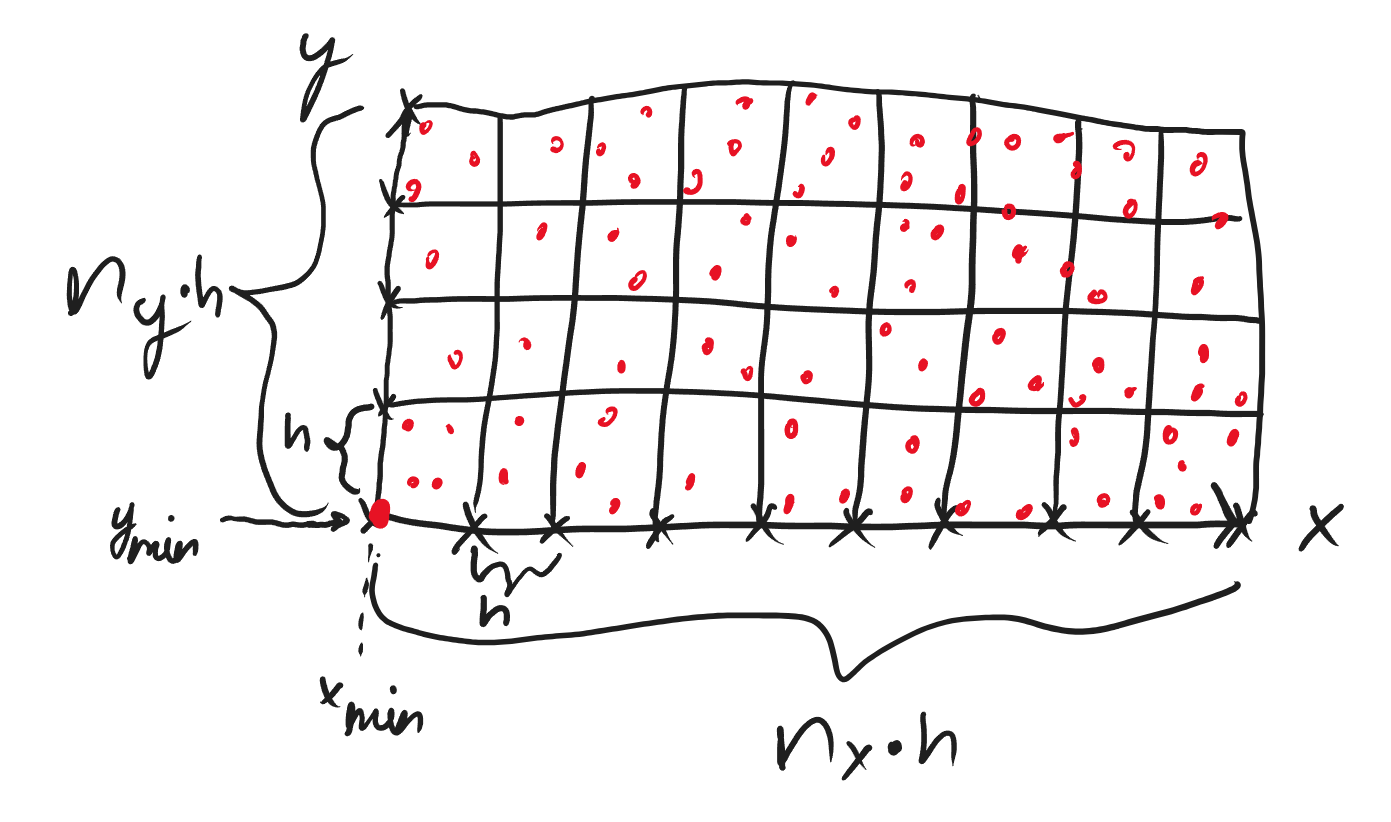
\includegraphics[width = .4\textwidth]{figs/PointGrid.png}
	\caption{Illustrasjon av røde punkter i et regulært rutenett i \(xy\)-planet.}
\end{figure}
For å kunne visualisere punktskyen som en sammenhengende overflate, så konstruerer jeg et regulært rutenett i \(xy\)-planet med dimensjoner \(\textbf{width} = x_{\text{max}} - x_{\text{min}}\) og \(\textbf{height} = y_{\text{max}} - y_{\text{min}}\). Hvor \(x_{\text{max}}\), \(x_{\text{min}}\), \(y_{\text{max}}\) og \(y_{\text{min}}\) er henholdsvis største og minste verdi for \(x\)- og \(y\)-koordinatene til punktene. Jeg velger så at hver rute i det regulære rutenettet er et kvadrat med areal \(\SI{10}{\metre\squared}\) (steglengde \(h = \SI{10}{\metre}\)), slik at \(n_{x} = \lceil \textbf{width}/h \rceil\) og \(n_{y} = \lceil \textbf{height}/h \rceil\) er henholdsvis antall ruter i \(x-\) og \(y-retning\). Hvert punkt kan så sorteres inn i ruten som dekker \(x\)- og \(y\)-koordinatene dens ved å regne ut rad- og kolonneindeks \(i\) og \(j\) i rutenettet som
\begin{align*}
	i &= \lfloor \frac{x - x_{\text{min}}}{h} \rfloor \\
	j &= \lfloor \frac{y - y_{\text{min}}}{h} \rfloor.
\end{align*}
For hver rute kan det regnes ut en gjennomsnittlig \(z\)-koordinat ved å ta gjennomsnittet av \(z\)-koordinatene til alle punktene med tilsvarende rad- og kolonneindeks
\begin{align*}
	\bar{z}_{i,j} &= \frac{1}{n_{i,j}}\sum_{k = 0}^{n_{i,j}}z_{i,j,k},\text{ eller for tomme ruter }
	\bar{z}_{i,j} = \frac{1}{8}\sum_{k=i-1}^{i+1}\sum_{\substack{l=j-1 \\ k\neq i \lor l\neq j}}^{j+1} \bar{z}_{k,l}.
\end{align*}
hvor \(n_{i,j}\) er antall punkter innenfor ruten som tilsvarer rad \(i\) kolonne \(j\). Gjennomsnittshøyden i en tom rute regnes som gjennomsnittet av gjennomsnittshøydene til naborutene \parencite[ss.140-141]{nylundMAT301MatematikkIII2023}.
Hvis dette må regnes for en rute på kanten av rutenettet, så må man ekskludere de ikke-eksisterende naboene.
Settet med regulært fordelte punkter kan så sentreres rundt origo, og skrives til fil på formatet
\begin{align*}
	&n_{x}\cdot n_{y} \\
	&(i\cdot h - n_{x}\cdot h/2,\quad \bar{z}_{i,j} - (z_{\text{max} - z_{\text{min}}})/2,\quad j\cdot h - n_{y}\cdot h/2) \\
	&...
\end{align*}
for alle \(j=0,1,2,...,n_{y}-1\) for alle \(i=0,1,2,...,n_{x}-1\). Første linjen i filen inneholder antall punkter. Videre er hver koordinat translatert slik at origo er sentrert, og \(y\)- og \(z\)- koordinaten er byttet om for innlesning i Unity \parencite{UnityEngine2023} som bruker et venstrehendt koordinatsystem med positiv \(y\)-akse som oppoverretning. Se \hyperref[ap:vert]{'Utdrag av vertices.txt'} for eksempel på resulterende punktdata.

\subsubsection{Indeksering}
For å kunne tegne en trekantflate av de regulært fordelte punktene i underseksjonen '\hyperref[M:1:1]{Vertekser}', så må det konstrueres en regulær triangulering med punktene som vertekser i trekanter \parencite[ss.140-141]{nylundMAT301MatematikkIII2023}. Dette gjøres ved å ta for seg kvadratet med hjørner \(v_{0} = j + i\cdot n_{y}\), \(v_{1} = (j+1) + i\cdot n_{y}\), \(v_{2} = j + (i+1)\cdot n_{y}\) og \(v_{3} = (j+1) + (i+1)\cdot n_{y}\), hvor \(\vec{v}_{k}\) er de regulært fordelte punktene, og \(j=0,1,2,...,n_{y}-1\) for alle \(i=0,1,2,...,n_{x}-1\).
\begin{figure}[H]
	\centering
	\begin{subfigure}{.5\textwidth}
		\centering
		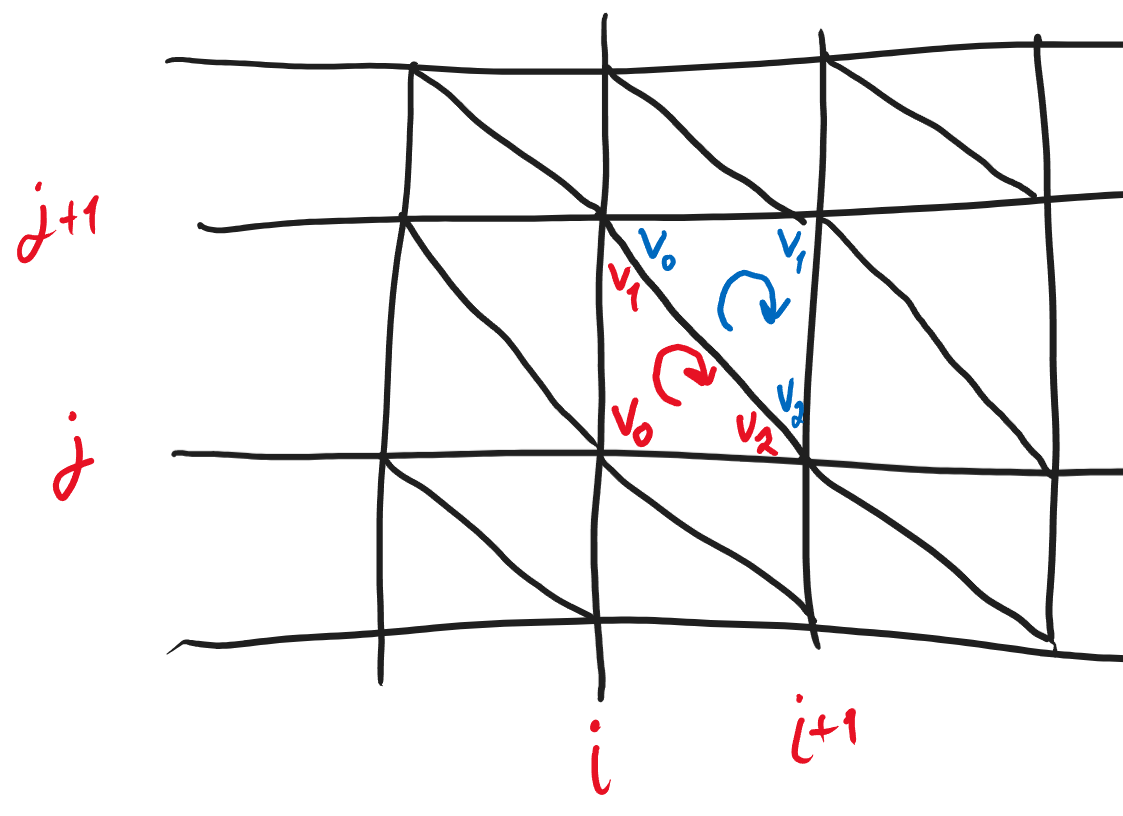
\includegraphics[width=.6\linewidth]{figs/Indices.png}
		\caption{Indeksering av vertekser i trekanter.}
	\end{subfigure}%
	\begin{subfigure}{.5\textwidth}
		\centering
		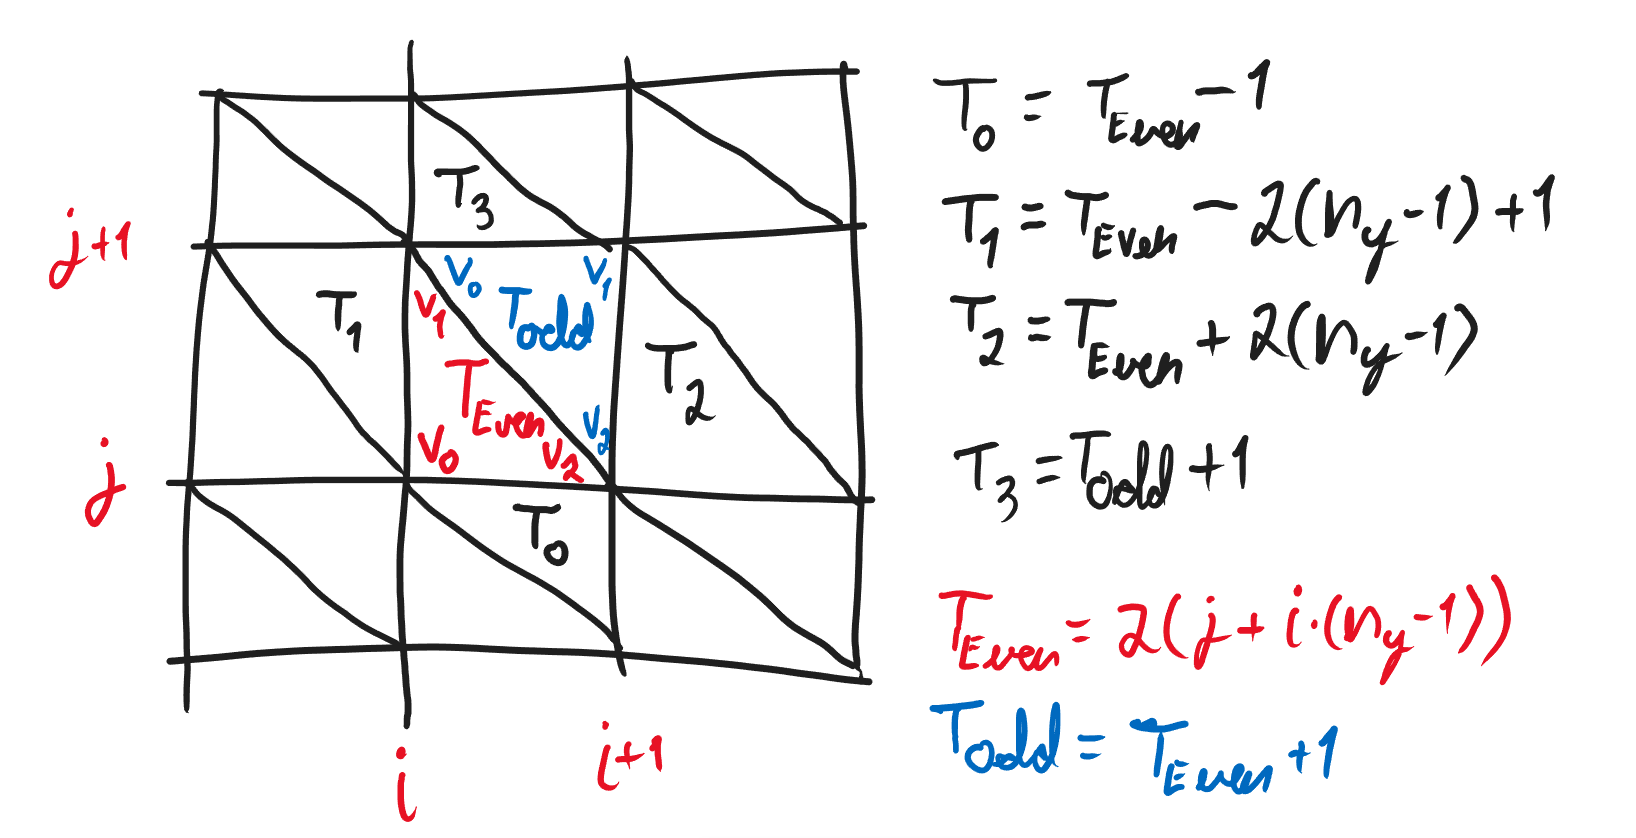
\includegraphics[width=\linewidth]{figs/Neighbours.png}
		\caption{Indeksering av nabotrekanter.}
	\end{subfigure}
	\caption{Illustrasjon av indeksering av trekanter og naboinformasjon per kvadrat i rutenettet. Trekantene er indeksert med klokka fordi de skal brukes i Unity sitt venstrehendte koordinatsystem.}
\end{figure}
Videre er det to trekanter \(T_{\text{even}}\) og \(T_{\text{odd}}\) per kvadrat med henholdsvis partallsindeks og oddetallsindeks.
Altså kan området deles opp i \((n_{x}-1)\cdot (n_{y}-1)\) antall kvadrater med en partallstrekant
\begin{align*}
 	T_{\text{even}} &= 2(j + i\cdot (n_{y}-1)), \qquad T_{\text{odd}} = T_{\text{even}} + 1.
\end{align*} 
Indeksering med naboinformasjon kan skrives til fil på formen
\begin{align*}
	&2(n_{x}-1)\cdot (n_{y}-1) \\
	& v_{0}\text{ } v_{1}\text{ } v_{2}\text{ } T_{\text{odd}}\text{ } T_{0}\text{ } T_{1} \\
	& v_{1}\text{ } v_{2}\text{ } v_{3}\text{ } T_{2}\text{ } T_{\text{even}}\text{ } T_{3} \\
	&...
\end{align*}
Hvor første linje er totalt antall trekanter, og hvert par med linjer etter holder indekser og naboinformasjon for partall- og oddetallstrekanter i for et vilkårlig kvadrat. Se \hyperref[ap:vert]{'Utdrag av indices.txt'} for eksempel på resulterende indekseringsdata.

\subsection{Ball på trekantflate}
For å simulere baller lagde jeg klassen \verb+BallPhysics+ som legges til som komponent på en instance av Unitys innebygde sfære-primitiv. Klassen har en referanse til \verb+TriangleSurface+-objektet den skal rulle på. Videre definerer jeg parametere for ballens masse \([\si{\kilogram}]\), radius \([\si{\metre}]\), friksjon [dimensjonsløs] og bounciness [dimensjonsløs].

\subsubsection{Kollisjonsdeteksjon} \label{sec:3:A}
For å dettektere kollisjon med trekantflaten, så vil ballen kalle \verb+GetCollision+-metoden i \verb+TriangleSurface+ objektet i hver \verb+FixedUpdate+. Ballen gir da posisjonen til senteret sitt \(p\) til \verb+TriangleSurface+, som bruker barysentriske koordinater til å finne trekanten ballen er på \parencite[ss.78-79]{nylundMAT301MatematikkIII2023}. Videre finner \verb+TriangleSurface+ punktet \(s\) på trekanten som er på linje med senteret i ballen langs \(y\)-aksen.

\begin{figure}[H]
	\centering
	\label{fig:kollisjon}
	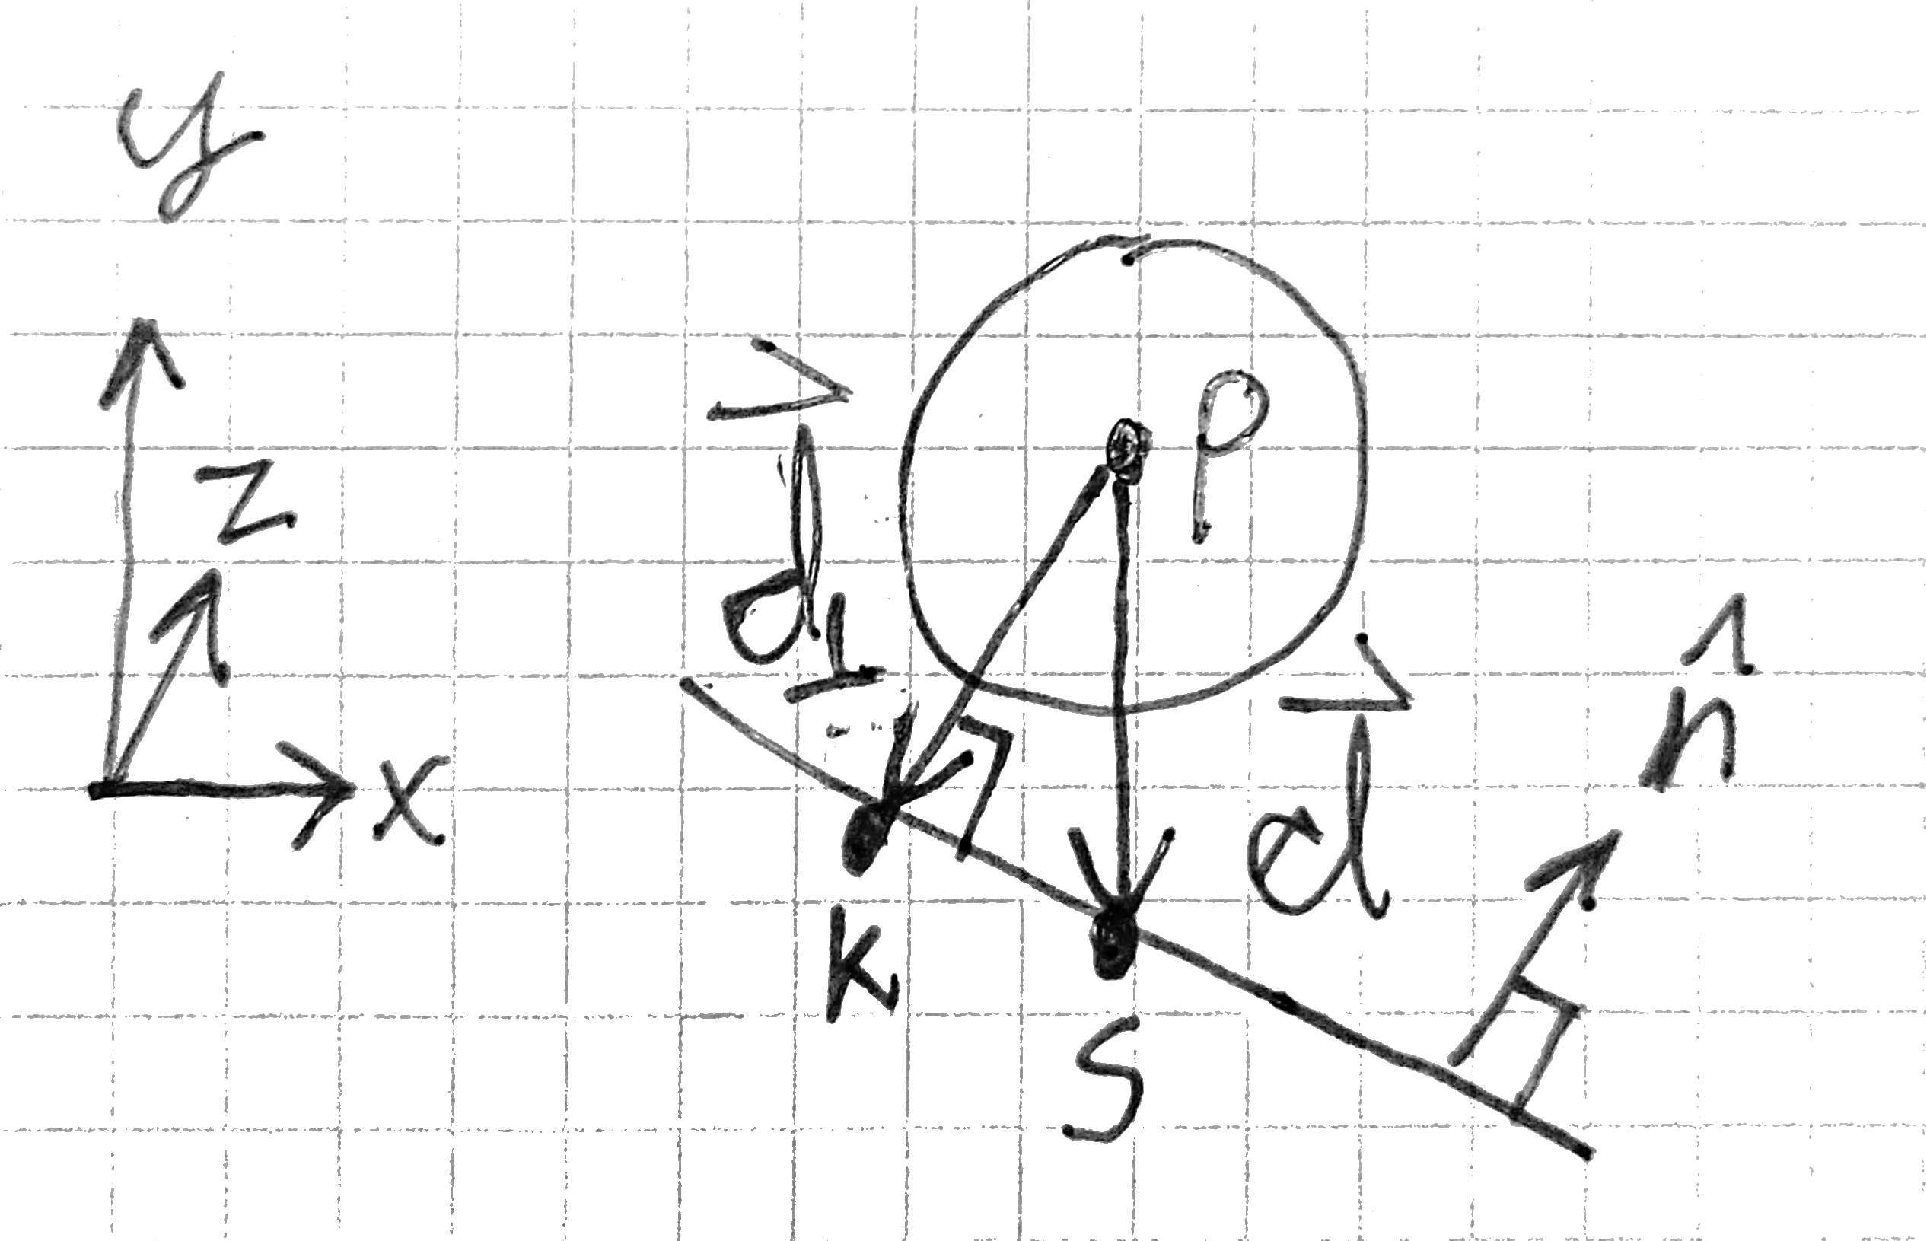
\includegraphics[scale=0.25]{figs/kollisjon.pdf}
	\caption{Diagram av kollisjonsdeteksjon. \(p\) er posisjonen til ballens senter, \(s\) er punktet på flaten med samme \(x\)- og \(z\)-koordinat som ballens senter, og \(k\) er punktet på flaten nærmest ballens senter.}
\end{figure}

For å sjekke om ballen er i kontakt med flaten beregner jeg først punktet \(k\) på flaten som er nærmest ballens senter \(p\)
\begin{align*}
	k &= p + \left(\vec{(s-p)}\cdot\hat{n}\right)\hat{n},
\end{align*}
og sjekker om differansen \(|p - k|\) er mindre eller lik radiusen \(r\) til ballen. I tilfellet hvor \(|p-k|\leq r\), så er det kollisjon. For å unngå at ballen beveger seg gjennom kollisjonsflaten setter jeg så ballens posisjon til å være i radius avstand fra kontaktpunktet langs enhetsnormalen
\begin{align*}
	p_{\text{korrigert}} &= k + r\cdot\hat{n}.
\end{align*}
For å simulere spretting endrer jeg ballens hastighet til å bli
\begin{align*}
	\vec{v}_{\text{etter}} &= \vec{v}_{\text{før}} - \left(1+b\right)\left(\vec{v}_{\text{før}}\cdot\hat{n}\right)\hat{n},
\end{align*}
hvor \(b\in [0,1]\) er bounciness-parameteren til ballen, og representerer hvor stor brøkdel av normalkomponenten av hastigheten som skal reflekteres ved kollisjon. For \(b = 0\) så mister ballen all hastighet normalt på planet. Hvis \(b=1\) så vil ballen få like stor hastighet normalt på planet som før kollisjonen, men i motsatt retning.

\subsubsection{Glidefysikk}
For å simulere fysikken på ballen, så finner jeg først alle kreftene på ballen i både tilfellet når den er og ikke er i kontakt med trekantflaten.
\begin{figure}[H]
	\centering
	\label{fig:frilegmediagram}
	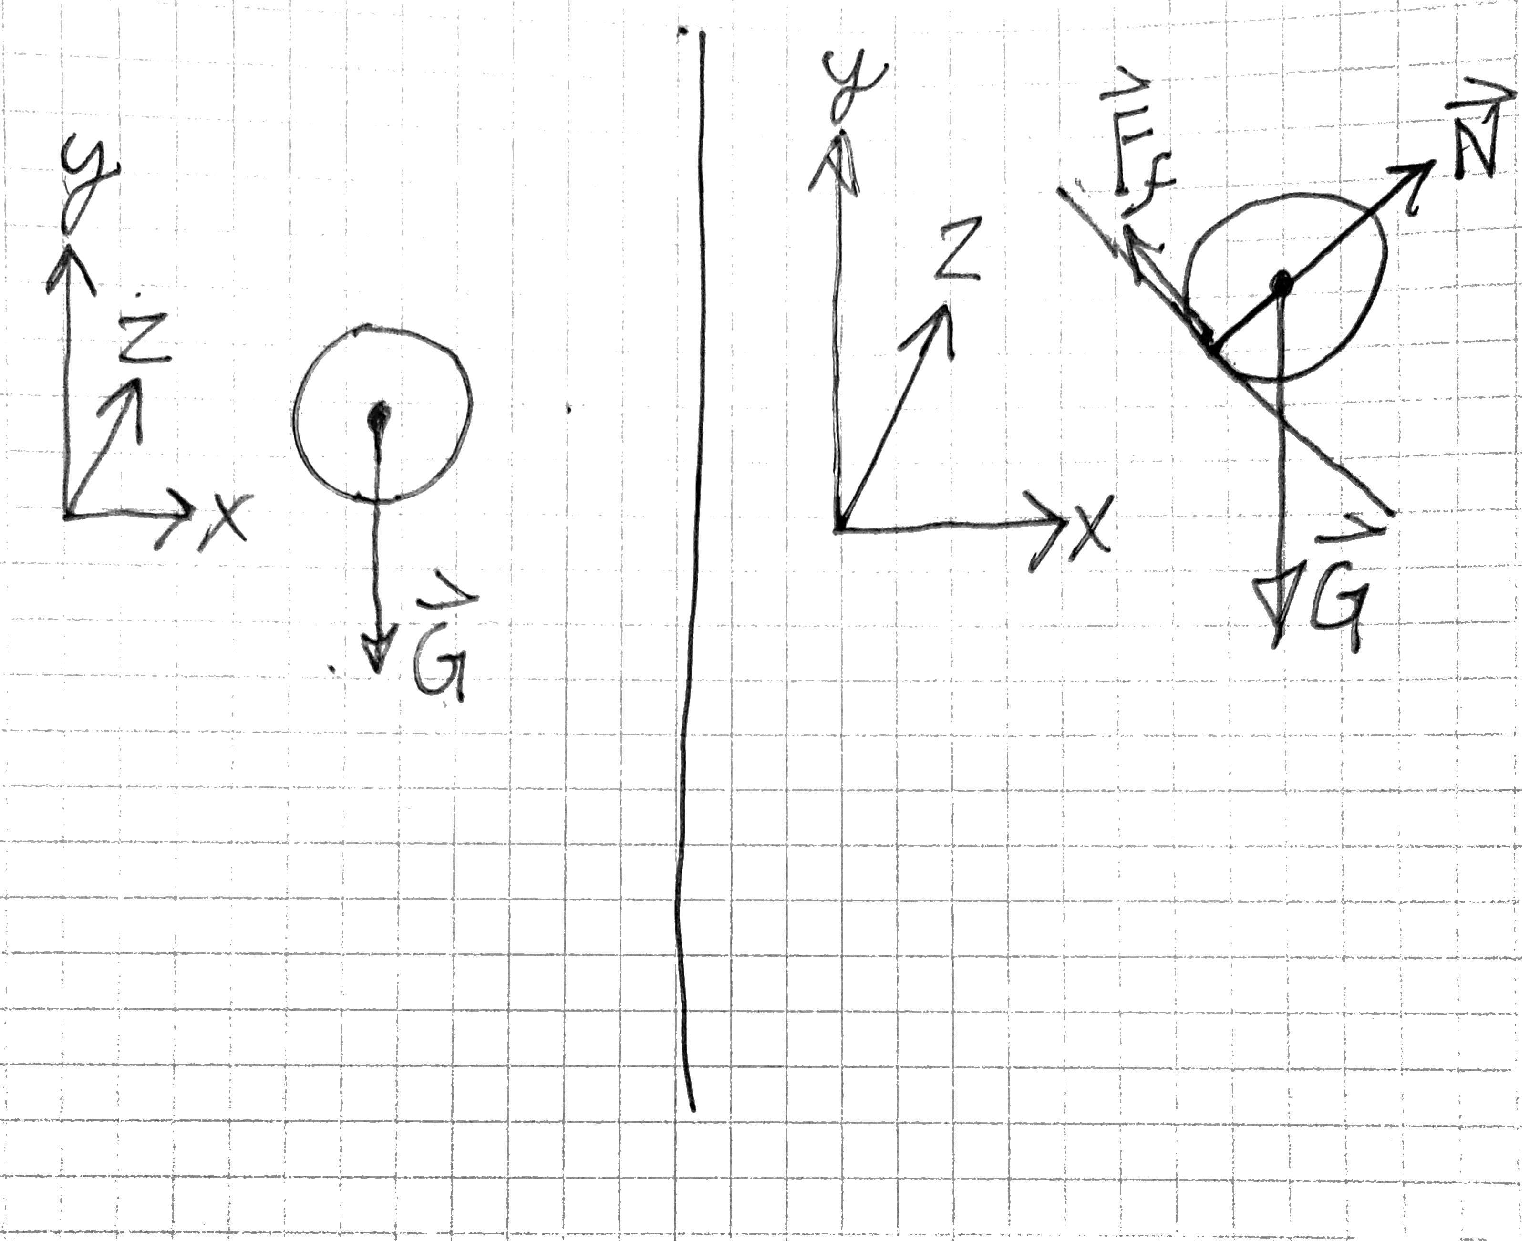
\includegraphics[scale=0.25]{figs/frilegmediagram.pdf}
	\caption{Frilegmediagram av ballen i både fritt fall, og på trekantflaten, med Unity sitt venstrehendte koordinatsystem tegnet inn.}
\end{figure}

I begge tilfeller er tyngdekraften på ballen lik
\begin{align*}
	\vec{G} &= m\vec{g} = m\left(\SI{-9.81}{\metre\per\second^{2}}\right)\uvecj
\end{align*}
hvor \(m\) er ballens masse i kilogram.

I tilfellet hvor ballen er i kontakt med trekantflaten, så opplever ballen en normalkraft
\begin{align*}
	\vec{N} &= -\left(\vec{G}\cdot\hat{n}\right)\hat{n},
\end{align*}
hvor \(\hat{n}\) er enhetsnormalvektoren til trekanten ballen er i kontakt med. Videre modelerer jeg også en glidefriksjonskraft
\begin{align*}
	\vec{F}_{f} &= -\mu |\vec{N}| \hat{v}_{\parallel}, \qquad
	\hat{v}_{\parallel} = \frac{\vec{v} - \left(\vec{v}\cdot\hat{n}\right)\hat{n}}{|\vec{v} - \left(\vec{v}\cdot\hat{n}\right)\hat{n}|}.
\end{align*}
hvor \(\mu\) er en kinetisk friksjonskonstant, og \(\vec{v}\) hastighetsvektoren til ballen. Friksjonskraften virker da alltid mot bevegelsesretningen langs flaten ballen er i kontakt med.

Jeg finner så akselerasjonen til ballen ved Newton's andre lov, slik at
\begin{align*}
	\vec{a} &= \frac{\vec{G}+\vec{N}+\vec{F}_{f}}{m},
\end{align*}
og integrerer hastighet \(\vec{v}\) og posisjon \(\vec{p}\) med Forward-Euler algoritmen
\begin{align*}
	\vec{v}_{t+\Delta t} &= \vec{v}_{t} + \vec{a}\cdot\Delta t, \\
	p_{t+\Delta t} &= p_{t} + \vec{v}_{t+\Delta t}\cdot \Delta t,
\end{align*}
Hvor \(\Delta t = \SI{0.02}{\second}\).

\subsubsection{Rulling på flere trekanter}
I tilfellet hvor ballen krysser fra en trekant til neste, så har jeg implementert to separate måter å håndtere det på. I tilfellet hvor ballen har en bounciness som er større enn \(0\), så håndteres all kollisjon med den delvise refleksjonen beskrevet i underseksjon '\hyperref[sec:3:A]{Kollisjonsdeteksjon}'
\begin{align*}
	\vec{v}_{\text{etter}} &= \vec{v}_{\text{før}} - \left(1+b\right)\left(\vec{v}_{\text{før}}\cdot\hat{n}\right)\hat{n}.
\end{align*}

I tilfellet hvor ballens bounciness er satt til å være \(0\), så bruker jeg i stedet en refleksjon av planet med normal lik gjennomsnittsnormalen til de to involverte trekantene \parencite[ss.120-124]{nylundMAT301MatematikkIII2023}.
\begin{align*}
	\vec{v}_{\text{etter}} &= \vec{v}_{\text{før}} - 2\left(\vec{v}_{\text{før}}\cdot\hat{n}\right)\hat{n},
	\qquad
	\hat{n} = \frac{\hat{n}_{\text{før}}+\hat{n}_{\text{etter}}}{|\hat{n}_{\text{før}}+\hat{n}_{\text{etter}}|}.
\end{align*}
Dette bevarer farten til ballen over trekantbyttet. Jeg har også valgt å kun gjøre denne refleksjonen i tilfellet hvor
\begin{align*}
	\left(\hat{n}_{\text{før}}\cross \hat{n}_{\text{etter}}\right)\cdot\left(\hat{n}_{\text{før}}\cross \hat{v}_{\parallel}\right) < 0,
\end{align*}
hvor \(\hat{v}_{\parallel}\) er enhetsvektoren i samme retning som komponenten av ballens hastighet som er parallel med trekanten.
Betingelsen over, sørger for at hastigheten kun er bevart over konvekse skjøter relativt til positiv \(y\)-retning, slik at ballen kan komme i fritt fall hvis den sklir utfor et fall.
\begin{figure}[H]
	\centering
	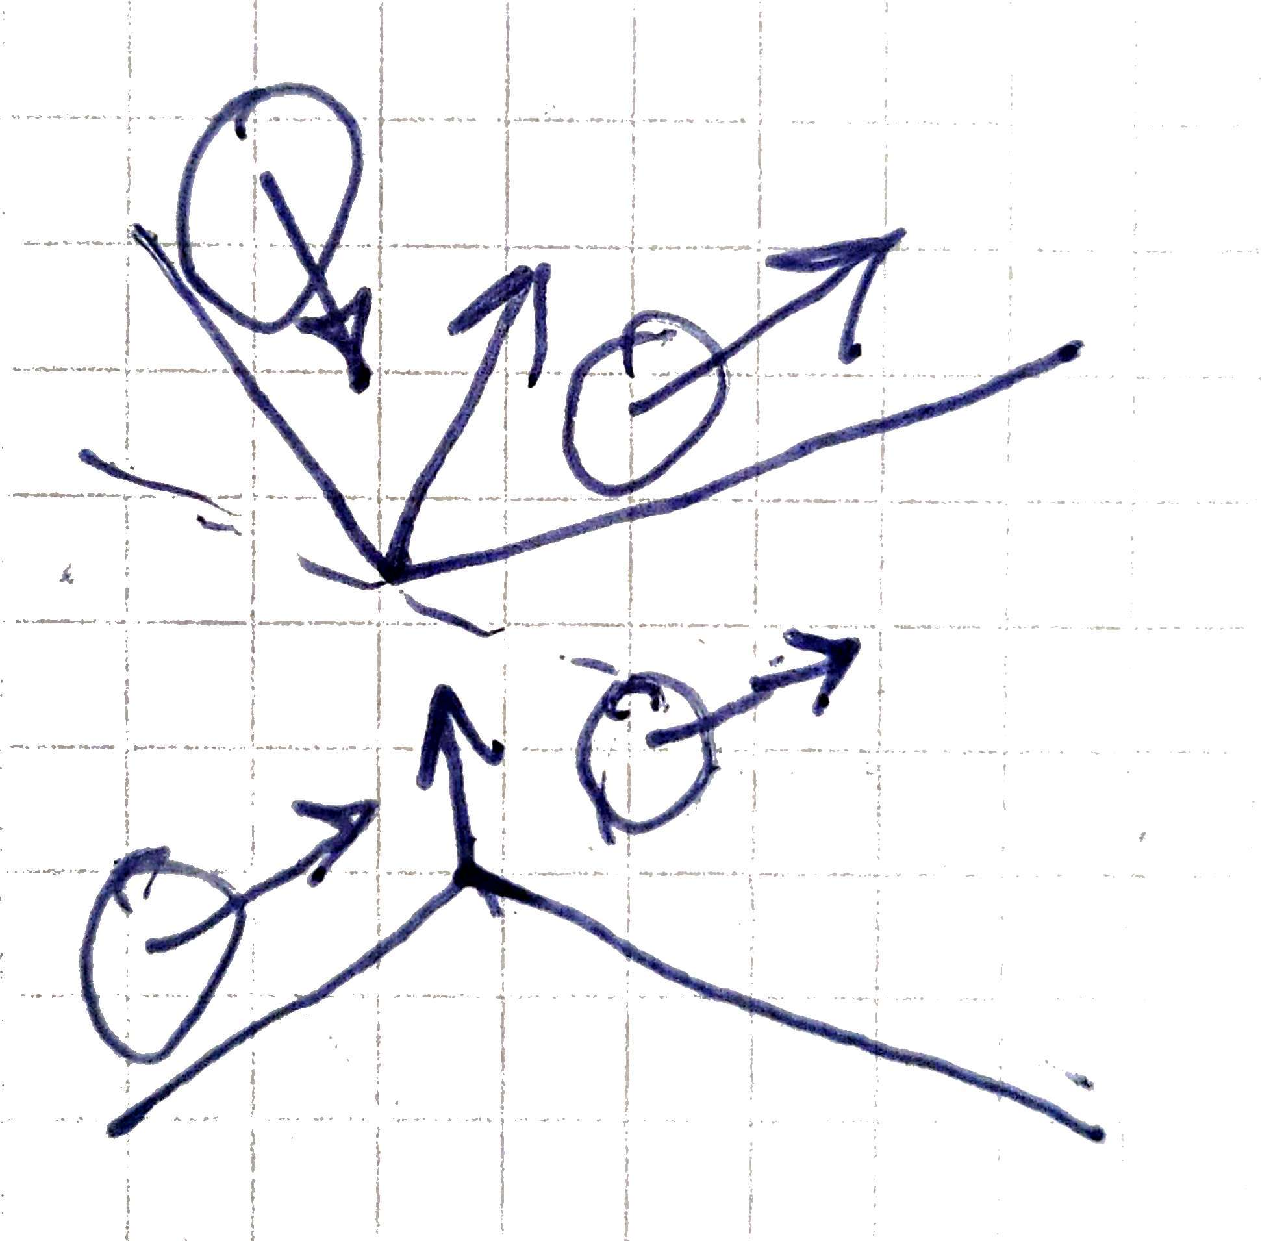
\includegraphics[width=.25\textwidth]{figs/refleksjon.pdf}
	\caption{Korrigering av hastighetsretning ved konvekse, men ikke konkave skjøter. Positiv \(y\)-akse rettet oppover på figuren.}
\end{figure}

\subsection{B-Splines og simulering av vassdrag}
For å simulere vassdrag som produseres under ekstremnedbør, modelerer jeg et sett med enkeltregndråper i form av baller som følger fysikken beskrevet i forrige sekjson. Videre får hver ball en tilfeldig generert startposisjon innenfor et valgt volum over terrenget. Jeg velger så å lagre posisjonen til hver av regndråpene \(15\) gjevnt fordelte ganger over en tidsperiode på \(\SI{30}{\second}\). De lagrede posisjonene blir så brukt som kontrollpunkter i \(xz\)-planet for en \(2D\) kvadratisk B-Spline, implementer med deBoors algoritme \parencite[ss.98-102]{nylundMAT301MatematikkIII2023}, som skal representere enkeltdråpenes bevegelse horisontalt. Splinen kan så tegnes ved å evaluere punkter for \(750\) uniformt fordelte verdier av parameteren \(t\), som jeg tegner rette linjer mellom. De tegnede punktene løftes opp på terrengoverflaten ved å beregne høyde med barysentriske koordinater.

For å simulere effekten av et slik vassdrag på en kampestein eller annet løsmateriale, så bruker jeg likningen for motstandskraft i fluid
\begin{align*}
	\vec{F}_{D} &= \frac{1}{2}C_{D}\rho A |\vec{v}|\vec{v},
\end{align*}
hvor \(C_{D}\) er dragkoeffisienten til legemet som påvirkes, \(\rho = \SI{1000}{\kilogram\per\metre\cubed}\) er tettheten til fluidet, \(A\) er tversnittarealet som står normalt på fluidets bevegelsesretning, og \(\vec{v} = \vec{v}_{f} - \vec{v}_{b}\) er fluidets hastighet relativt til legemet \parencite[s.7]{alexanderMovingBouldersFlash2016}. I min simulasjon bruker jeg en ball med masse \(m_{b} = \SI{50}{\kilogram}\) og radius \(r_{b} = \SI{1}{\metre}\) plasert på terrenget. Jeg har valgt en dragkoeffisient på \(C_{D} = 0.5\) siden det gjelder for sfærer i mange forskjellige typer flyt \parencite{hallDragSphere2023}. Videre har ballen et tversnittareal \(A = \pi r_{b}^{2}\).
Hastighetsvektoren til fluidet regner jeg ut som
\begin{align*}
	\vec{v}_{f} = v\hat{T}_{\text{mean}}, \qquad v = \SI{3}{\metre\per\second},
\end{align*}
Hvor \(v\) er en konstant hastighet jeg har valgt for vassdraget, og \(\hat{T}_{\text{mean}}\) er den gjennomsnittet av enhetstangentvektoren i nærmeste punkt på hver B-Spline innenfor en radius på \(\SI{5}{\metre}\) fra ballen. Jeg tilnærmer tangentvektoren \(\vec{T} = S(t+\Delta t) - S(t)\) for en parameterverdi \(t\) som et lite steg \(\Delta t = 0.5\) langs splinen \(S\). For å finne parameterverdien tilsvarende nærmeste punkt \(P_{c}\) for posisjonen til ballen \(P_{b}\) på splinen \(S\), så bruker jeg at
\begin{align*}
  	\vec{(P_{b} - P_{c})}\cdot\vec{T_{c}} = 0,
\end{align*}
som jeg kan tilnærme en løsning for iterativt med Newton's midtpunktsmetode
\begin{figure}[H]
	\centering
	\begin{subfigure}{.5\textwidth}
		\centering
		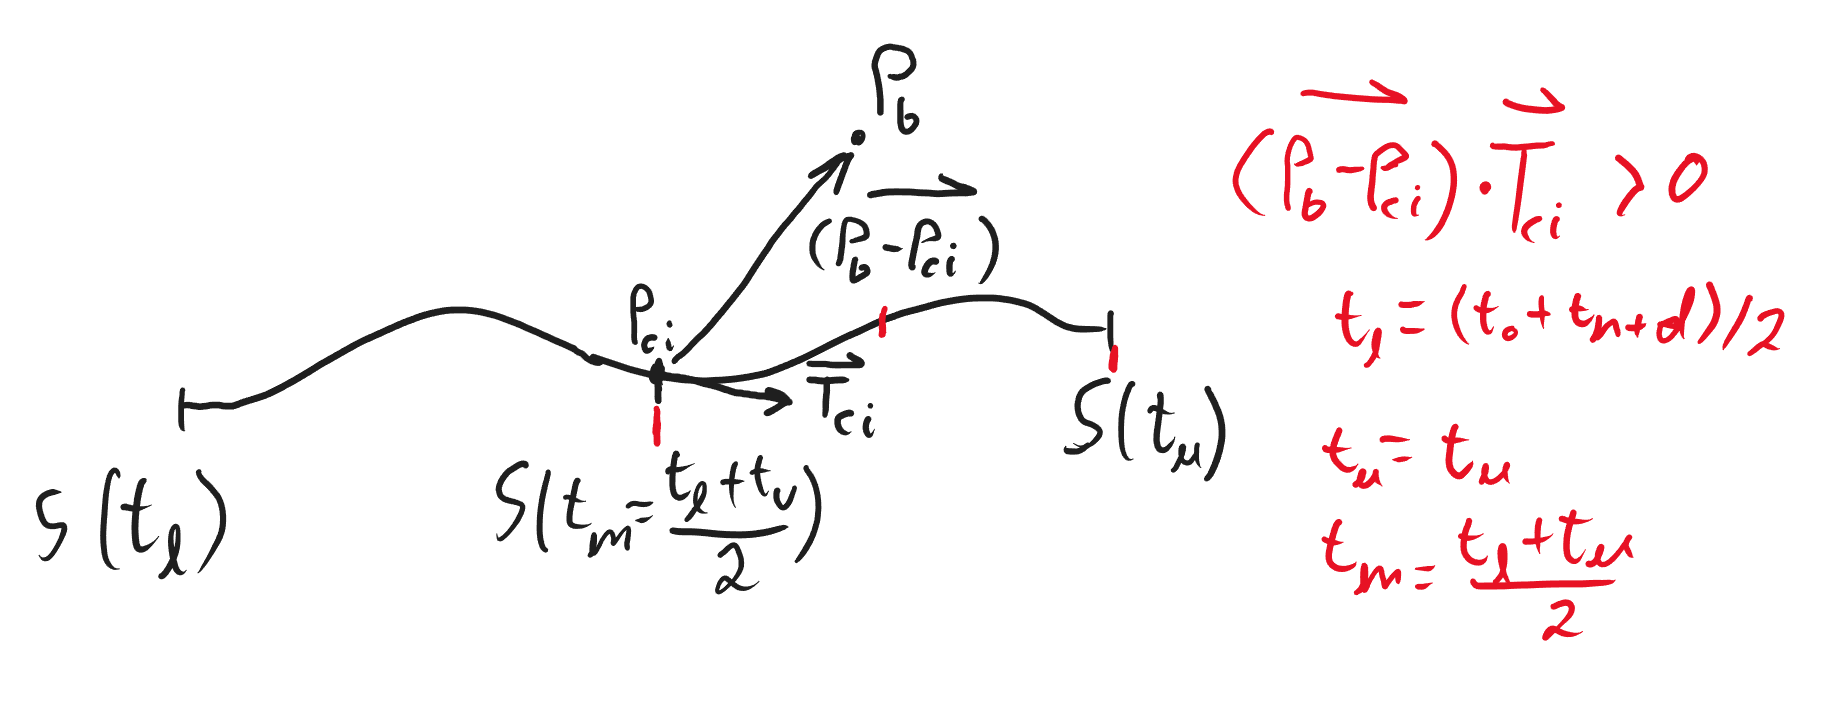
\includegraphics[width=.9\linewidth]{figs/newtonPos.png}
		\caption{Velger øvre interval hvis prikkproduktet er positivt.}
	\end{subfigure}%
	\begin{subfigure}{.5\textwidth}
		\centering
		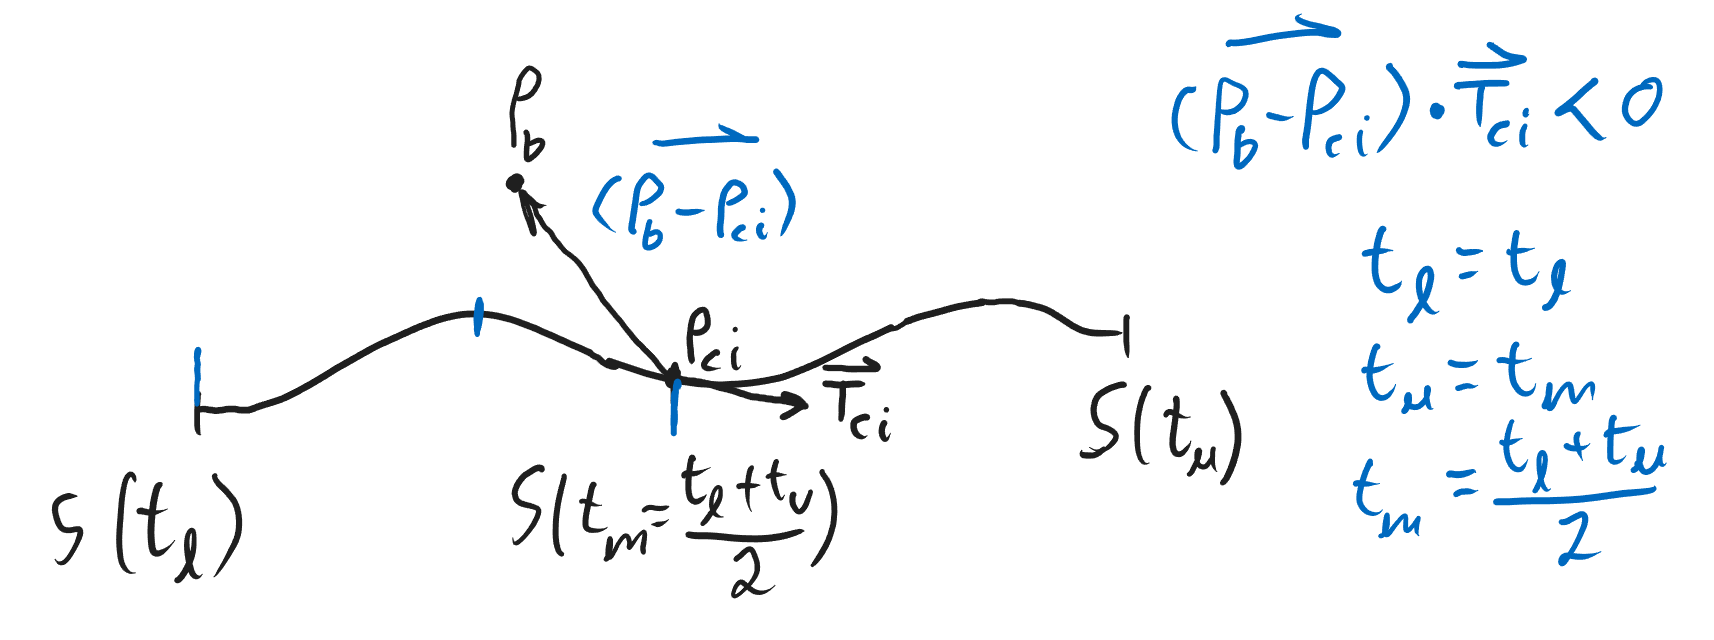
\includegraphics[width=.9\linewidth]{figs/newtonNeg.png}
		\caption{Velger nedre interval hvis prikkproduktet er negativt.}
	\end{subfigure}
	\caption{Iterativ inskrenkning av parameterverdi for punkt \(P_{c,i}\) på splinen \(S\) som er nærmest punktet \(P_{b}\).}
\end{figure}

\section{Resultater}
\subsection{Punktsky og glatting} \label{fig:punkt}
\begin{figure}[H]
	\centering
	\begin{subfigure}{.5\textwidth}
		\centering
		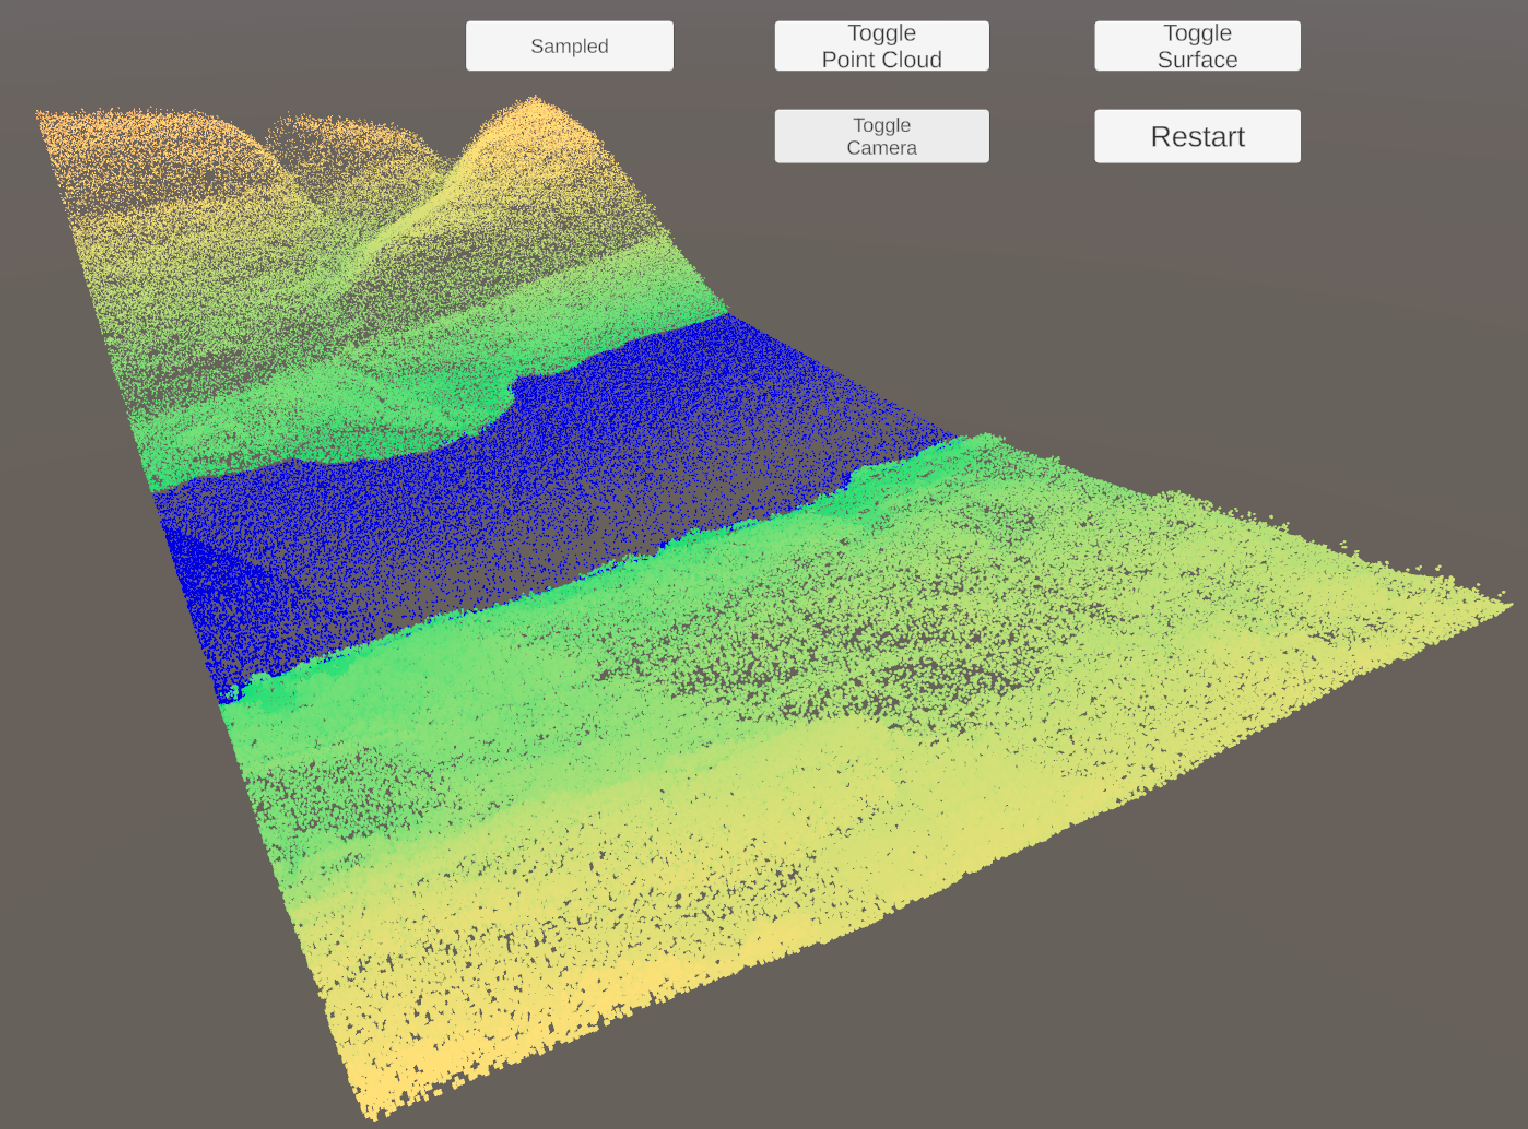
\includegraphics[width=.9\linewidth]{figs/punktSample.png}
		\caption{Hvert hundrede punkt fra rådataene.}
	\end{subfigure}%
	\begin{subfigure}{.5\textwidth}
		\centering
		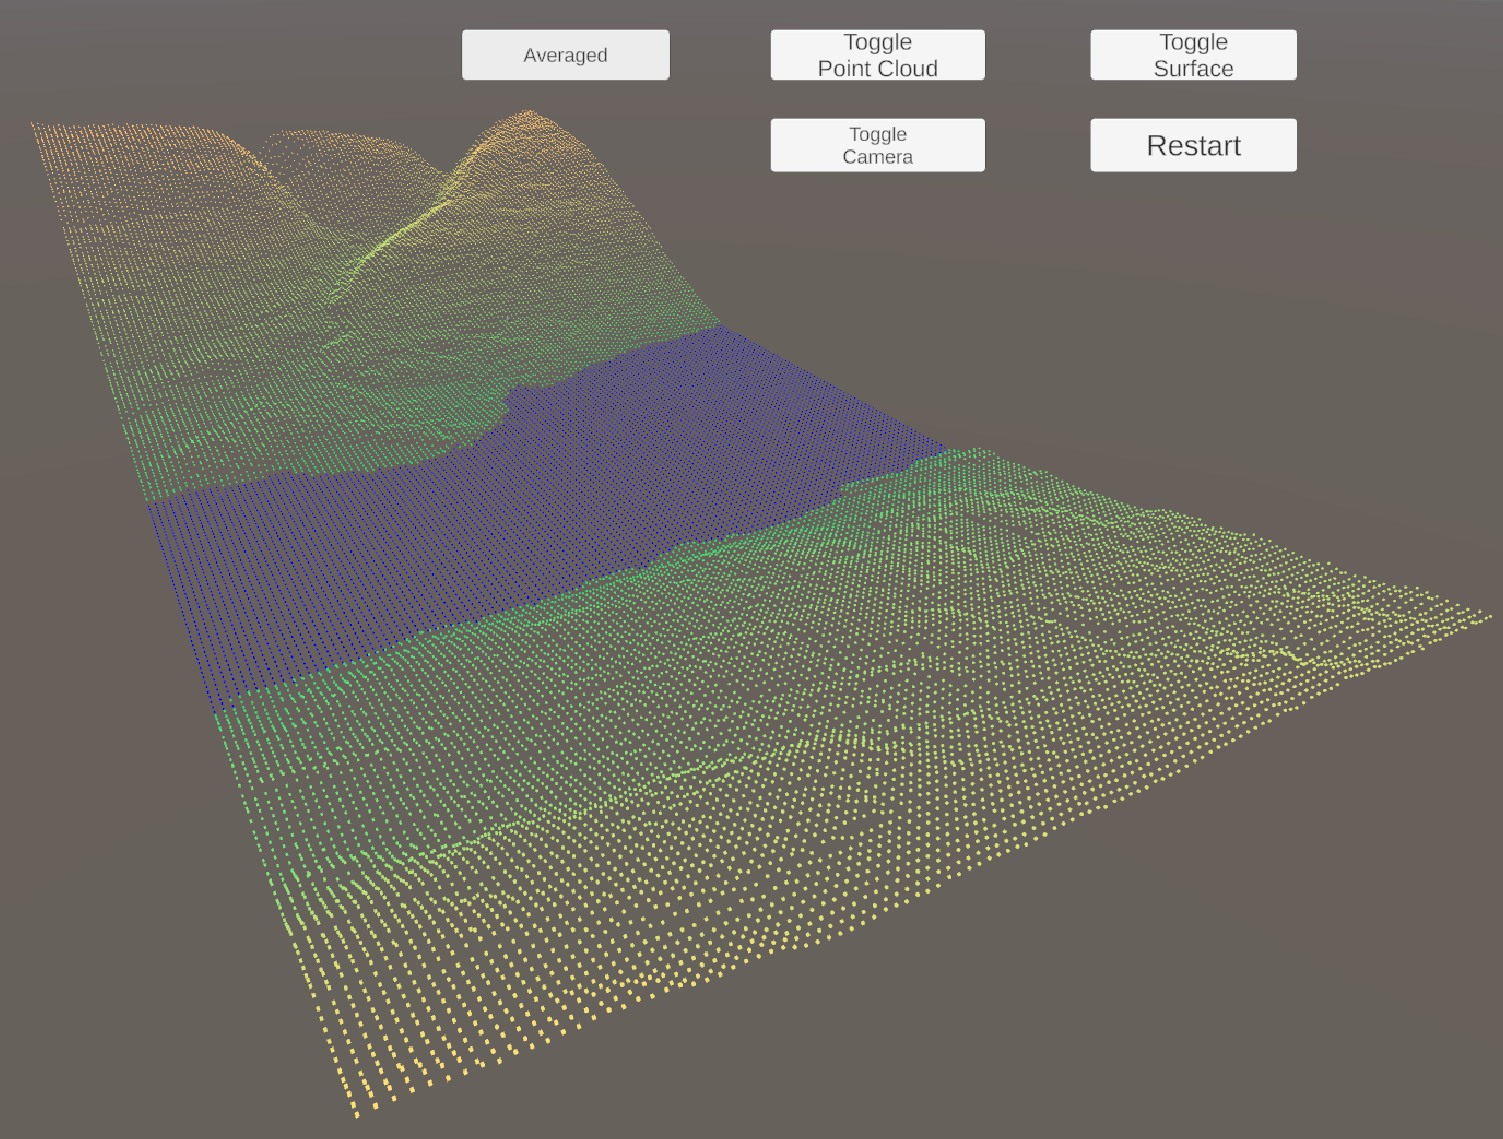
\includegraphics[width=.9\linewidth]{figs/punktMean.png}
		\caption{Regulært glattede punkter.}
	\end{subfigure}
	\caption{Plott av punktskydataene.}
\end{figure}

\subsection{Overflate og ball} \label{fig:ball}
\begin{figure}[H]
	\centering
	\begin{subfigure}{.5\textwidth}
		\centering
		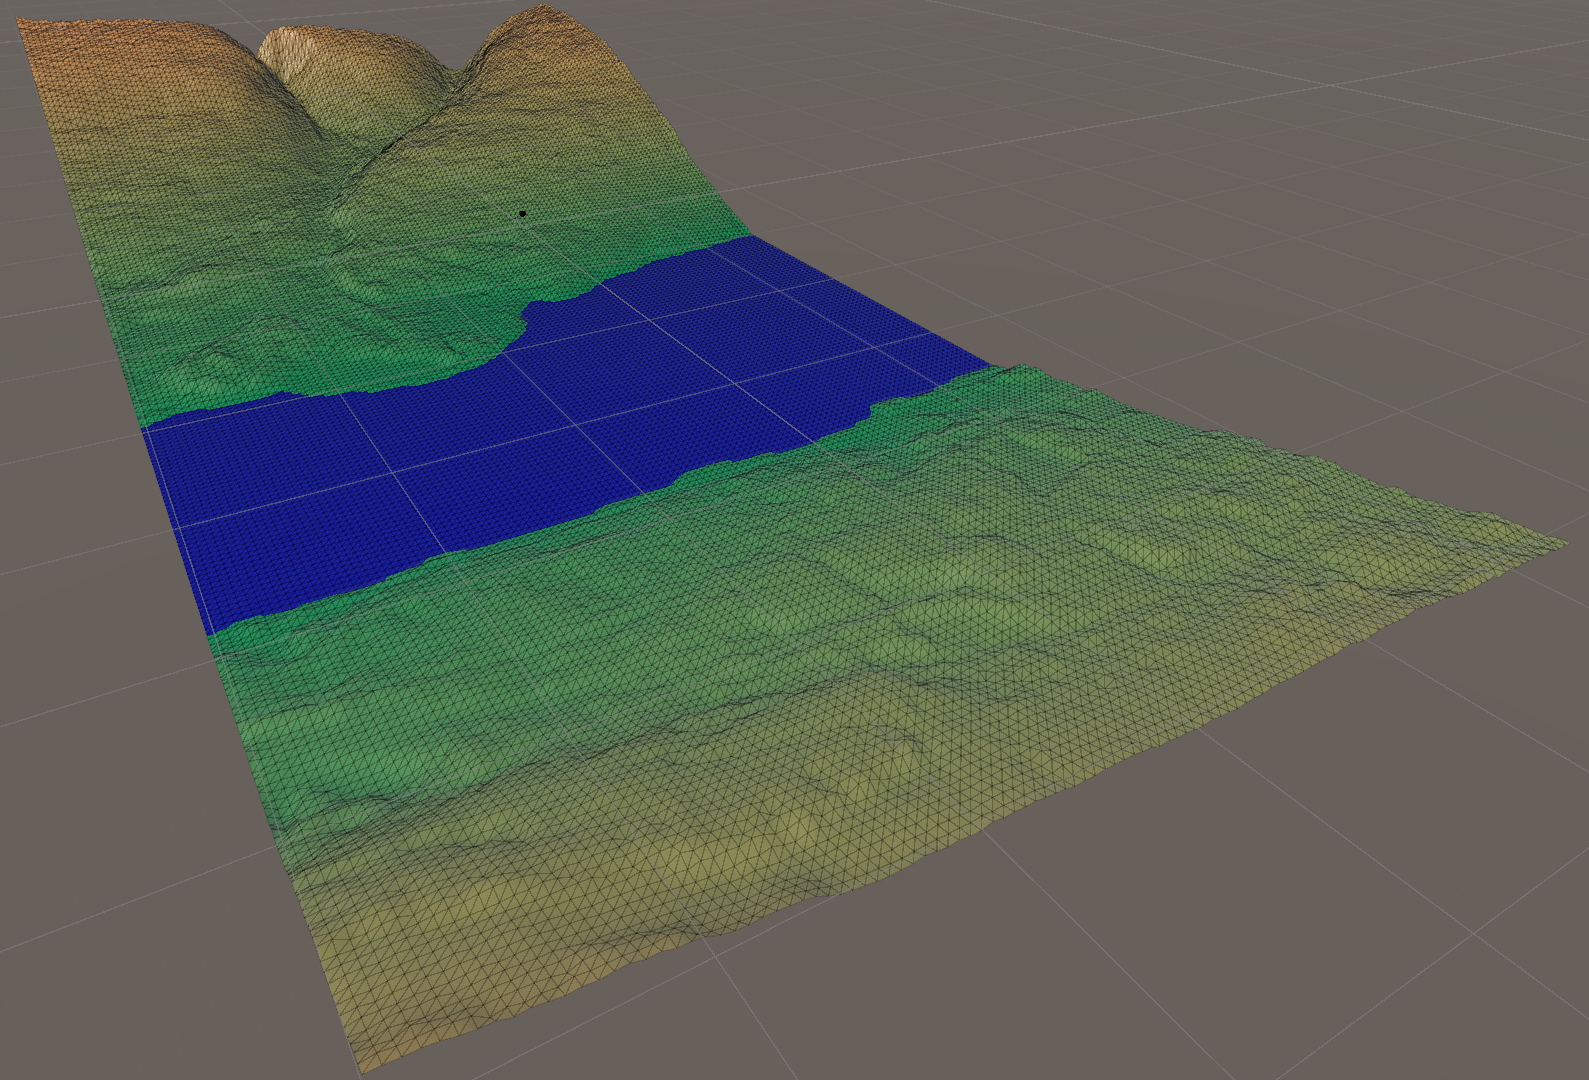
\includegraphics[width=.9\linewidth]{figs/surfaceGrid.png}
		\caption{Regulært indeksert trekantflate}
	\end{subfigure}%
	\begin{subfigure}{.5\textwidth}
		\centering
		\includegraphics[width=\linewidth]{figs/BallPåFlate.png}
		\caption{Oransj ball som sklir på flaten.}
	\end{subfigure}
	\caption{Plott av trekantflaten og to perspektiver av samme ball.}
\end{figure}

\subsection{Spline og vassdrag} \label{fig:regn}
\begin{figure}[H]
	\centering
	\begin{subfigure}{.5\textwidth}
		\centering
		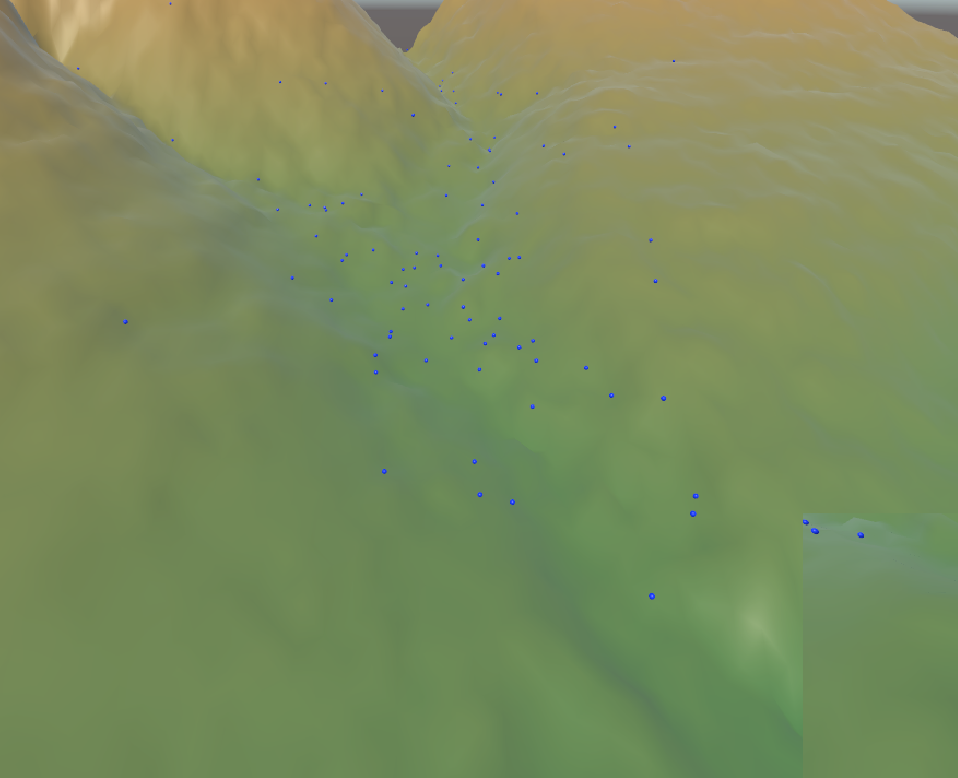
\includegraphics[width=.9\linewidth]{figs/rain.png}
		\caption{Regndråper simulert som små, blå baller.}
	\end{subfigure}%
	\begin{subfigure}{.5\textwidth}
		\centering
		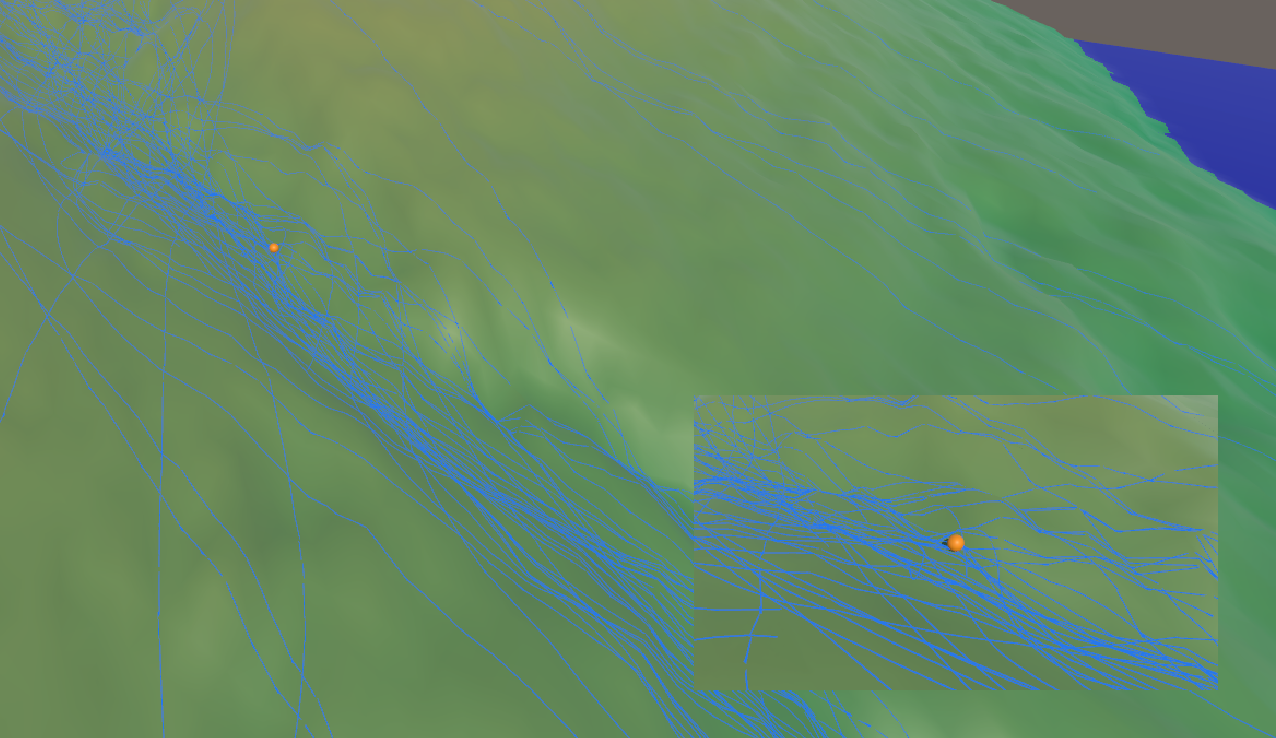
\includegraphics[width=\linewidth]{figs/water.png}
		\caption{B-Splines som viser vassdrag forårsaket av regn.}
	\end{subfigure}
	\caption{Plott av regn og vassdrag. Den oransje ballen flyter med vassdraget.}
\end{figure}

\begin{table}[H] \label{tab:fps}
	\centering
	\begin{tabular}{|l|r|}
		\hline
		Antall splines & Bildefrekvens \\\hline
		\(100\) & \(167\) fps \\\hline
		\(250\) & \(53\) fps \\\hline
		\(500\) & \(4\) fps \\\hline
	\end{tabular}
	\caption{Antall B-Splines (1 per regndråpe simulert), og tilsvarende gjennomsnitlig bildefrekvens.}
\end{table}

\section{Diskusjon}
\subsection{Punktsky}
Fra  \hyperref[fig:punkt]{figur 7} ser jeg at punktskydataene er blitt prossesert riktig. Delfigur \hyperref[fig:punkt]{(a)} viser vært hundrede av punktene innlest fra textfilen som LASzip genererte fra .laz-filen med rådata. Det er totalt \(318905\) punkter som rendres. Fargen er satt basert på høyden i vertex-shaderen 'GPUInstancing.shader'. Dataene er som forventet ugjevnt fordelt i det horisontale planet, og har varierende tetthet.  Delfigur \hyperref[fig:punkt]{(b)} viser de regulært glattede verteksene generert av \verb+PointCloudSurfaceParser.cpp+, og er som forventet gjevnt fordelt i det horisontale planet med konstant tetthet innenfor området.

\subsection{Flate og ball}
\hyperref[fig:ball]{Figur 8} viser den regulært indekserte trekantflaten generert av \verb+PointCloudSurfaceParser.cpp+, og at en ball kan plaseres og bevege seg på trekantflaten.

\subsection{Spline og vassdrag}
Som illustrert i \hyperref[fig:regn]{Figur 9}, så er \(100\) individuelle regndroper i stand til å trille på trekantflaten samtidig. Dette kan brukes for å simpelt og raskt estimere hvor regn kommer til å flyte langs terrenget. Videre vises B-Splinene som visualiserer det estimerte vassdraget som antas følges av videre nedbør. Ballen som representerer løsmateriale blir fraktet med vassdraget og, basert på start posisjon, kan ende opp i bunnen av dalen som terrenget viser, eller bli sittende fast på veien på grunn av friksjonen på \(\mu = 0.04\) for ballen.

Valget om å simulere retningen til vassdraget med tangentvektoren til B-Splinene er mindre enn optimalt ettersom algoritmen for å finne parameterverdiene for nærmeste punkt per spline skalerer dårlig for økt antall spliner, som vist i \hyperref[tab:fps]{Tabell 1}. Aktuelle alternativer er å bruke en felt- eller diffusjonsbasert fluidsimmulering til å bestemme hastighetsvektorer per kvadrat i det regulære rutenettet som ligger til grunne for trekantflaten. En slik simulasjon hadde også antagelig kunne modellere et vassdrag med hastighet som varierer i rommet.
 
\section{Konklusjon}
Hensikten med dette prosjektet var å utforske konstruksjonen av trekantflater fra punktsky-måling av terreng, til en mulig modell for simulering av vassdrag og effekt av nedbør på løsmateriale. Konstruksjonen av trekantflate er fult mulig, og gir et modellert tereng som kan brukes til simulering av vær.

Valgt metode for visualisering av vassdrag og simmulering av flom er ikke egnet for fysisk komplekse situasjoner grunnet at ytelsen raskt går ned når man øker antall regndråper. Derimot er modellen aktuelt som verktøy for enkle visualiseringer av effekten av regn på enkeltlegmer.

\newpage
\printbibliography

\appendix
\section{Prosjektfiler} \label{ap:1}
Prosjektet er tilgjengelig her: \url{https://github.com/FunkMarvel/VisSimMappe.git} .

All kode for prossesering av punktskydata er tilgjengelig i PointCloudSurfaceParser-undermappen i Git repoet,

\url{https://github.com/FunkMarvel/VisSimMappe/tree/e58f43b7870e46e7956c186ae735f39589018496/PointCloudSurfaceParser}

All kode for Unity-simuleringen er tilgjengelig i VisSimMappeUnityProsjekt-undermappen av Git repoet,

\url{https://github.com/FunkMarvel/VisSimMappe/tree/e58f43b7870e46e7956c186ae735f39589018496/VisSimMappeUnityProsjekt}

\subsection{Utdrag av vertices.txt} \label{ap:vert}
\begin{verbatim}
28800
(-600, 87.3003, -300)
(-600, 86.173, -295)
(-600, 84.6683, -290)
(-600, 82.7369, -285)
(-600, 81.8657, -280)
(-600, 83.2463, -275)
(-600, 81.257, -270)
(-600, 79.8496, -265)
(-600, 79.406, -260)
(-600, 79.7682, -255)
(-600, 78.7479, -250)
(-600, 79.5409, -245)
(-600, 80.1995, -240)
(-600, 78.4865, -235)
...
\end{verbatim}

\subsection{Utdrag av indices.txt} \label{ap:idx}
\begin{verbatim}
56882
0 1 120 1 -1 -1
1 121 120 238 0 2
1 2 121 3 1 -1
2 122 121 240 2 4
2 3 122 5 3 -1
3 123 122 242 4 6
3 4 123 7 5 -1
4 124 123 244 6 8
4 5 124 9 7 -1
5 125 124 246 8 10
5 6 125 11 9 -1
6 126 125 248 10 12
6 7 126 13 11 -1
7 127 126 250 12 14
...
\end{verbatim}

\end{document}